\documentclass[11pt]{article}

\usepackage[margin=1in]{geometry}
\usepackage{amsmath,amssymb,bm}
\usepackage{booktabs}
\usepackage{graphicx}
\usepackage{subcaption}
\usepackage{hyperref}
\usepackage{xcolor}
\usepackage{enumitem}
\usepackage{microtype}
\usepackage{array}

\graphicspath{{figures/}}

\hypersetup{
  colorlinks=true,
  linkcolor=blue!50!black,
  citecolor=blue!50!black,
  urlcolor=blue!50!black
}

\title{Motion-Aware Extension of POV-SLAM for Semi-Static and Dynamic Object-Level SLAM in 2D Simulation}
\author{Simulation Research Prototype}
\date{\today}

\newcommand{\Static}{\textsc{Static}}
\newcommand{\SemiStatic}{\textsc{Semi-Static}}
\newcommand{\Dynamic}{\textsc{Dynamic}}
\newcommand{\SEtwo}{\mathrm{SE}(2)}
\newcommand{\Rtwo}{\mathbb{R}^{2}}
\newcommand{\Normal}{\mathcal{N}}
\newcommand{\Uniform}{\mathcal{U}}

\begin{document}
\maketitle

\begin{abstract}
Long-term robot autonomy requires maps that remain useful when objects move, disappear, or reappear. POV-SLAM addresses this problem for semi-static environments by combining object-level landmarks with probabilistic consistency reasoning in a factor-graph SLAM framework. However, POV-SLAM is primarily motivated by objects that change between revisits, not by continuously moving objects that can persistently corrupt landmark-based localization during a traversal. This report presents a simulation-only research prototype that implements a simplified POV-SLAM-style baseline and a motion-aware extension. The extension augments the object-level map with a three-state motion layer, classifying objects as \Static, \SemiStatic, or \Dynamic. Static and semi-static objects are retained as localization and map evidence, while dynamic objects are excluded from stationary landmark updates and tracked separately using a constant-velocity Kalman filter. In 2D indoor simulation experiments, the motion-aware variants improve average absolute trajectory error relative to the simplified POV-SLAM-style baseline under mixed, semi-static-only, dynamic-fraction stress, and observation-noise stress scenarios. The results suggest that explicitly separating continuous dynamics from semi-static map change is a useful extension of POV-SLAM-style object-aware SLAM, while also exposing limitations of the lightweight simulation backend.
\end{abstract}

\section{Introduction}
Classical SLAM methods often assume that the world is static. This assumption is fragile in long-term indoor deployments such as warehouses, labs, and service-robot environments, where boxes, carts, cones, and other movable objects may be relocated between visits or may move continuously during a robot traversal. Treating every observed object as a permanent landmark can bias the pose estimate and produce inconsistent maps. Treating every inconsistent observation as a pure outlier, however, discards information that may be valuable for change detection and scene understanding.

POV-SLAM, introduced by Qian et al.~\cite{qian2023povslam}, targets semi-static environments by using object-level reasoning and a probabilistic consistency model. The key insight is that object observations should not be forced into a binary decision of either perfectly static landmark or useless outlier. Instead, potentially changed objects can be represented using a Gaussian-uniform measurement model and optimized with variational expectation-maximization (EM), allowing the SLAM backend to jointly estimate robot pose, object landmarks, and object consistency.

This report builds on that idea, but focuses on a distinct failure mode: continuously dynamic objects. Semi-static changes occur across revisits; dynamic motion occurs during the traversal itself. A box moved overnight and a cart rolling across the robot's field of view should not be represented by the same state. The first is a candidate map update, while the second is a moving entity whose trajectory should be tracked separately and should not become a stationary landmark.

The contribution of this project is a simulation-only prototype that frames POV-SLAM as the baseline and introduces a motion-state extension. The system remains deliberately lightweight: it uses a 2D world, simulated object detections, nearest-neighbor association, a simplified object-level pose correction model, and a constant-velocity Kalman tracker. The purpose is not to reproduce the full POV-SLAM paper or to build a real robotics system. Instead, the goal is to show, in controlled simulation, that adding explicit dynamic-state reasoning to a POV-SLAM-style semi-static formulation can improve robustness when dynamic clutter is present.

\section{Background: POV-SLAM}
\subsection{Problem setting}
POV-SLAM addresses SLAM in semi-static environments, where objects may be moved, removed, or newly introduced over long timescales. The paper argues that this setting is not fully handled by either static-scene SLAM or dynamic-object filtering. Static-scene SLAM assumes that previously mapped landmarks remain valid. Dynamic-object SLAM typically detects objects that move between consecutive frames and removes or tracks them. Semi-static objects occupy a middle ground: they may remain fixed during a single traversal but differ between revisits.

Let the robot trajectory be a sequence of poses
\begin{equation}
    \mathbf{X} = \{\mathbf{x}_1, \ldots, \mathbf{x}_T\}, \quad \mathbf{x}_t \in \SEtwo,
\end{equation}
and let the object map be a set of object landmarks
\begin{equation}
    \mathbf{L} = \{\mathbf{l}_1, \ldots, \mathbf{l}_M\}, \quad \mathbf{l}_j \in \Rtwo.
\end{equation}
Each object observation associates a robot pose with an object-level measurement. In an object-aware SLAM abstraction, the observation can be represented as
\begin{equation}
    \mathbf{z}_{tj} = h(\mathbf{x}_t, \mathbf{l}_j) + \bm{\epsilon}_{tj},
\end{equation}
where $h(\cdot)$ is the sensor prediction function and $\bm{\epsilon}_{tj}$ is measurement noise. In a static world, the residual
\begin{equation}
    \mathbf{r}_{tj} = \mathbf{z}_{tj} - h(\mathbf{x}_t, \mathbf{l}_j)
\end{equation}
is assumed to follow a Gaussian distribution centered at zero. Semi-static change breaks this assumption: a residual may be large because the pose is wrong, because the measurement is noisy, or because the object itself has changed.

\subsection{Object consistency as a latent variable}
The important modeling idea in POV-SLAM is to introduce a latent object consistency variable. Rather than forcing all object measurements into the same Gaussian landmark model, POV-SLAM represents the possibility that an object observation may be inconsistent with the current map. A simplified view of the per-object measurement likelihood is
\begin{equation}
    p(\mathbf{z}_{tj} \mid \mathbf{x}_t, \mathbf{l}_j, c_j)
    = c_j \Normal(\mathbf{r}_{tj}; \mathbf{0}, \Sigma)
    + (1-c_j) \Uniform(\mathbf{r}_{tj}; \Omega),
    \label{eq:pov_mixture}
\end{equation}
where $c_j \in [0,1]$ represents the probability that object $j$ is consistent with the map. The Gaussian component models normal landmark observations. The uniform component models large residuals caused by changed or unreliable objects. This is often called a Gaussian-uniform bimodal likelihood.

The consistency probability is not only a measurement weight; it is a semantic statement about the map. A high value of $c_j$ means the object is likely reliable as a landmark. A low value means the object may have changed or should not strongly constrain the pose graph. In the full POV-SLAM formulation, this consistency is estimated probabilistically and updated within a variational EM procedure.

\subsection{Variational EM interpretation}
The full POV-SLAM system uses a factor graph and a variational EM strategy to jointly reason about poses, landmarks, and object consistency. A simplified interpretation is as follows. The objective can be written as a maximum a posteriori problem over robot poses, landmarks, and latent object-consistency variables:
\begin{equation}
    \max_{\mathbf{X}, \mathbf{L}, \mathbf{c}} \; p(\mathbf{X}, \mathbf{L}, \mathbf{c} \mid \mathbf{Z}, \mathbf{U}),
\end{equation}
where $\mathbf{Z}$ are object observations and $\mathbf{U}$ are odometry measurements. Directly optimizing this posterior is difficult because the consistency variables create mixture factors. Variational EM separates the problem into two alternating steps:
\begin{enumerate}[leftmargin=*]
    \item \textbf{E-step:} estimate the posterior responsibility or belief that each object observation is consistent with the map.
    \item \textbf{M-step:} optimize poses and landmarks using the consistency-weighted measurement factors.
\end{enumerate}

In a practical weighted least-squares view, an observation receives a reliability weight
\begin{equation}
    w_{tj} \approx \frac{c_j \Normal(\mathbf{r}_{tj};\mathbf{0},\Sigma)}{c_j \Normal(\mathbf{r}_{tj};\mathbf{0},\Sigma) + (1-c_j)\Uniform(\mathbf{r}_{tj};\Omega)}.
\end{equation}
The SLAM optimizer then minimizes a weighted residual objective:
\begin{equation}
    \min_{\mathbf{X}, \mathbf{L}} \sum_t \|\mathbf{e}^{\mathrm{odom}}_t\|^2_{\Sigma_u^{-1}}
    + \sum_{t,j} w_{tj}\|\mathbf{r}_{tj}\|^2_{\Sigma_z^{-1}}.
\end{equation}
This view captures the intuition needed for the present prototype: consistent objects strongly constrain localization, while inconsistent objects are downweighted rather than naively trusted.

\subsection{What POV-SLAM gives us}
POV-SLAM is a strong baseline because it already improves over a static landmark assumption. Its central strengths are:
\begin{itemize}[leftmargin=*]
    \item \textbf{Object-level semantics:} objects are not only geometric features; they are named, persistent map entities.
    \item \textbf{Probabilistic consistency:} map-object reliability is estimated rather than hard-coded.
    \item \textbf{Semi-static robustness:} objects that move between revisits can be treated as unreliable or changed without immediately destroying the pose estimate.
    \item \textbf{Map interpretability:} the method produces object-level reasoning about reliable and unreliable scene components.
\end{itemize}

However, the paper's main problem setting is semi-static change. It does not focus on a three-way distinction between static landmarks, semi-static relocated objects, and continuously dynamic objects. This distinction motivates our extension.

\section{Motion-Aware Extension}
\subsection{Motivation}
A semi-static object and a dynamic object both produce large residuals, but for different reasons. A semi-static object may be stable in the current visit and useful after relocation is confirmed. A dynamic object violates the stationary landmark assumption at every frame while it moves. If both are represented only as low-consistency landmarks, the system loses an important distinction:
\begin{equation}
    \text{changed but stable} \neq \text{continuously moving}.
\end{equation}

The theoretical improvement is to refine POV-SLAM's object reliability layer into a motion-state layer. Instead of a single consistency concept, each object is assigned a state
\begin{equation}
    s_j \in \{\Static, \SemiStatic, \Dynamic\}.
\end{equation}
This state determines how the object participates in localization, mapping, and tracking.

\subsection{State-dependent interpretation}
The proposed state model uses the following semantics:
\begin{itemize}[leftmargin=*]
    \item \Static: the object is a trusted long-term landmark and receives high measurement weight.
    \item \SemiStatic: the object may move between revisits but is usually stable within a traversal; it receives moderate weight and may trigger a relocation update after repeated evidence.
    \item \Dynamic: the object moves continuously during traversal; it is excluded from stationary landmark updates and tracked separately.
\end{itemize}

This decomposes the single POV-SLAM consistency question, ``Is this object reliable with respect to the old map?'', into two questions: ``Is this object stable enough to localize against now?'' and ``Should this object be represented as a stationary map landmark?'' The answers are not always identical. A newly moved box may become stable and useful after confirmation, while a moving cart should remain a track, not a landmark.

\subsection{Heuristic state classification}
The prototype uses lightweight, hand-crafted features rather than a learned classifier. For each object hypothesis or observation stream, it considers:
\begin{itemize}[leftmargin=*]
    \item residual magnitude relative to the stored landmark prediction,
    \item inter-frame displacement of associated detections,
    \item estimated velocity magnitude,
    \item observation persistence across frames,
    \item revisit consistency or repeated evidence at a new location,
    \item semantic class priors, e.g., carts and cones are more likely to be dynamic than shelves and pillars.
\end{itemize}

The classifier outputs a hard label in the current implementation, though the same structure could be extended to soft probabilities
\begin{equation}
    p(s_j) = \{p(\Static), p(\SemiStatic), p(\Dynamic)\}.
\end{equation}

\subsection{Dynamic object tracking}
Objects classified as dynamic are routed to a constant-velocity Kalman tracker. Each dynamic track has state
\begin{equation}
    \mathbf{y}_k = [x, y, v_x, v_y]^\top,
\end{equation}
with transition model
\begin{equation}
    \mathbf{y}_{k+1} =
    \begin{bmatrix}
    1 & 0 & \Delta t & 0 \\
    0 & 1 & 0 & \Delta t \\
    0 & 0 & 1 & 0 \\
    0 & 0 & 0 & 1
    \end{bmatrix}
    \mathbf{y}_k + \mathbf{q}_k.
\end{equation}
Detections update the position components through a linear measurement model. Tracks are associated with observations using nearest-neighbor class-compatible gating. Stale tracks are terminated when they are not updated for a configurable number of frames.

The important design choice is that dynamic tracks are maintained as a sidecar representation. They explain moving objects and support qualitative visualization and tracking metrics, but they do not become static landmarks in the pose correction step. This mirrors the static/dynamic map separation used by dynamic SLAM systems such as DyOb-SLAM~\cite{wadud2022dyobslam}, while keeping the implementation small enough for a 2D simulation prototype.

\subsection{State-dependent SLAM weighting}
The motion-aware extension modifies the measurement weighting policy:
\begin{equation}
    w(s_j) =
    \begin{cases}
    w_{\mathrm{static}}, & s_j = \Static, \\
    w_{\mathrm{semi}}, & s_j = \SemiStatic, \\
    0, & s_j = \Dynamic.
    \end{cases}
\end{equation}
In the simplified implementation, dynamic objects are filtered from stationary landmark pose correction. Semi-static objects can contribute only when their observations are stable enough, and relocation is not confirmed from a single outlier. A relocation candidate is maintained and accepted only after repeated consistent observations in the new location.

This produces the central theoretical claim of the report:
\begin{quote}
A POV-SLAM-style consistency layer protects against semi-static changes, but it can still blur the distinction between changed objects and continuously moving objects. Adding a motion-state layer preserves the semi-static reasoning while preventing dynamic objects from entering the stationary map.
\end{quote}

\section{Prototype Implementation}
\subsection{Simulation environment}
The system is implemented as a 2D simulation-only research prototype. The world is a bounded rectangular indoor environment containing objects with unique identifiers, semantic class labels, radii, and motion types. Supported object categories include shelves, boxes, carts, cones, and pillars. Objects follow one of three behavior models:
\begin{itemize}[leftmargin=*]
    \item Static objects remain fixed for the full experiment.
    \item Semi-static objects remain fixed during a traversal but may relocate between revisits.
    \item Dynamic objects move continuously using simple velocity or waypoint-like behavior.
\end{itemize}

A robot traverses the map over multiple visits. The simulator produces ground-truth poses, noisy odometry, and object detections within a sensing radius and field-of-view abstraction. Each detection includes semantic label, confidence, and noisy object position.

\subsection{Baseline}
The baseline in this project is a simplified POV-SLAM-style method. It is not a full reproduction of Qian et al.'s factor graph or variational EM implementation. Instead, it captures the relevant baseline behavior for this simulation study:
\begin{itemize}[leftmargin=*]
    \item object observations are associated to persistent semantic landmarks;
    \item residuals between observations and stored landmarks are used to estimate consistency;
    \item inconsistent objects are downweighted using a Gaussian-like consistency score;
    \item repeated stable evidence may create or update a relocation candidate;
    \item no explicit continuous-dynamic object tracking is used.
\end{itemize}

Thus, the baseline represents the semi-static object-consistency philosophy of POV-SLAM, while the proposed method adds a distinct continuous-motion layer.

\subsection{Ablations}
Four methods are evaluated:
\begin{itemize}[leftmargin=*]
    \item \textbf{POV-style baseline:} semi-static consistency reasoning without dynamic tracking.
    \item \textbf{Dynamic filtering only:} adds dynamic object filtering but does not use the full dynamic track visualization and state layer.
    \item \textbf{Kalman tracking only:} adds sidecar dynamic tracking with the same localization behavior as filtering in the current lightweight backend.
    \item \textbf{Full motion-aware:} uses state classification, dynamic filtering, Kalman sidecar tracks, and semi-static update logic.
\end{itemize}

\section{Experiments}
\subsection{Scenarios}
The benchmark suite uses fixed random seeds and configuration-driven scenarios:
\begin{itemize}[leftmargin=*]
    \item \textbf{Semi-static only:} no continuously dynamic objects; some objects move between revisits.
    \item \textbf{Mixed:} static, semi-static, and dynamic objects are present together.
    \item \textbf{Dynamic-fraction stress:} the fraction of dynamic objects is swept from 0.0 to 0.65.
    \item \textbf{Noise stress:} object detection noise is swept from 0.15 to 0.50.
\end{itemize}

\subsection{Metrics}
The main localization metrics are absolute trajectory error (ATE) and relative pose error (RPE). Lower values are better. Map quality is measured using landmark position error, map consistency score, and false landmark updates. Object understanding is evaluated using state classification accuracy, confusion matrices, and change detection precision/recall. Tracking quality is represented by dynamic track position error, track survival length, and ID switches when available.

\subsection{Aggregate results}
Table~\ref{tab:aggregate_ate} summarizes the benchmark averages after replacing the original static-landmark baseline with the simplified POV-SLAM-style baseline. The strongest localization ablation is often dynamic filtering only, while the full motion-aware method adds the richer state and tracking outputs.

\begin{table}[t]
\centering
\caption{Average ATE across benchmark families. Lower is better. Values are from the current simulation prototype and should be interpreted as controlled simulation results, not real-robot performance.}
\label{tab:aggregate_ate}
\begin{tabular}{lrrrr}
\toprule
Scenario & POV baseline & Dynamic filter & Kalman tracking & Full motion-aware \\
\midrule
Mixed & 2.382 & \textbf{2.035} & \textbf{2.035} & 2.191 \\
Semi-static only & 1.983 & \textbf{1.881} & \textbf{1.881} & 1.886 \\
Dynamic-fraction stress & 2.173 & \textbf{1.890} & \textbf{1.890} & 1.897 \\
Noise stress & 2.427 & \textbf{2.046} & \textbf{2.046} & 2.171 \\
\bottomrule
\end{tabular}
\end{table}

The results support the main theory. A semi-static consistency baseline is robust to map changes, but it does not explicitly distinguish continuously moving objects from changed but stable landmarks. When dynamic clutter is present, filtering dynamic objects from stationary landmark correction improves localization robustness. The full motion-aware method is slightly behind the pure filtering ablation in some ATE aggregates because the current tracker is implemented as a sidecar rather than a full joint factor-graph variable. However, the full method is the more complete object-understanding system: it retains dynamic-object tracks and exposes state labels for visualization and diagnosis.

\subsection{Qualitative results}
Figure~\ref{fig:aggregate_plots} shows the aggregate ATE and classification plots generated by the benchmark scripts. Figure~\ref{fig:stress_plots} shows stress-test trends for increasing dynamic-object fraction and increasing detection noise. Figure~\ref{fig:qualitative} shows the full motion-aware qualitative map and confusion-matrix visualization.

\begin{figure}[t]
\centering
\begin{subfigure}{0.48\linewidth}
    \centering
    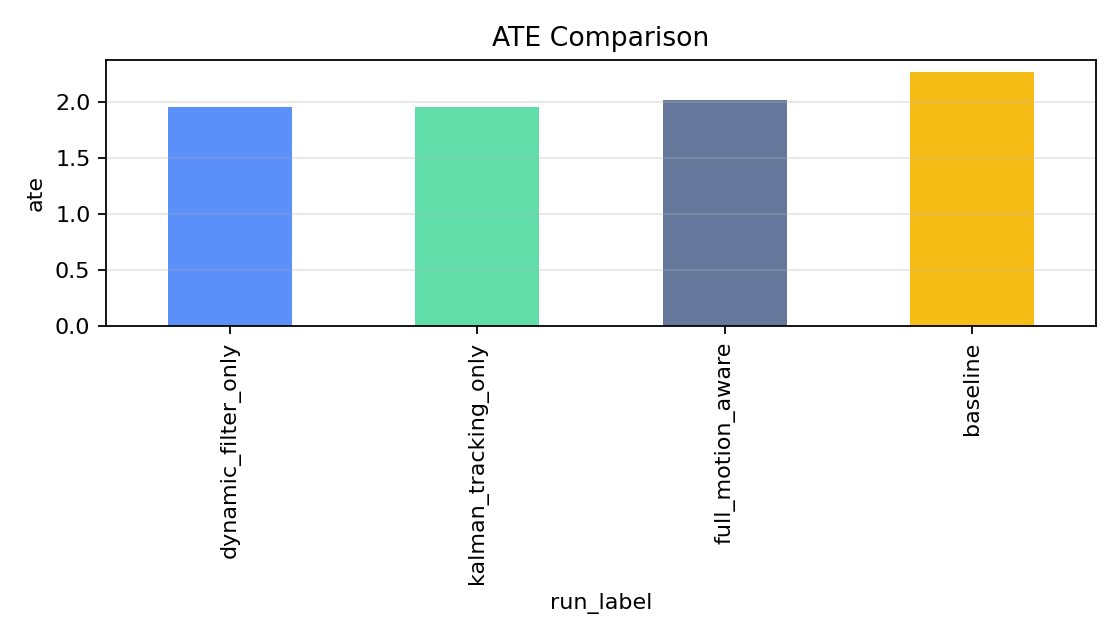
\includegraphics[width=\linewidth]{ate_comparison.png}
    \caption{ATE comparison.}
\end{subfigure}
\hfill
\begin{subfigure}{0.48\linewidth}
    \centering
    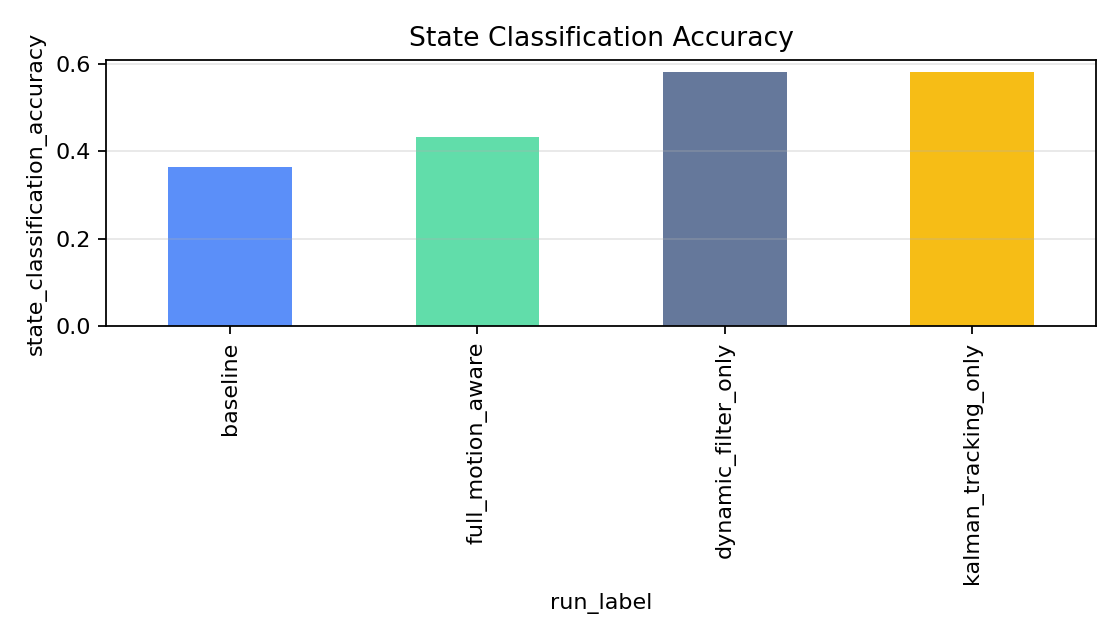
\includegraphics[width=\linewidth]{classification_accuracy.png}
    \caption{State classification accuracy.}
\end{subfigure}
\caption{Aggregate comparison figures produced by the benchmark pipeline.}
\label{fig:aggregate_plots}
\end{figure}

\begin{figure}[t]
\centering
\begin{subfigure}{0.48\linewidth}
    \centering
    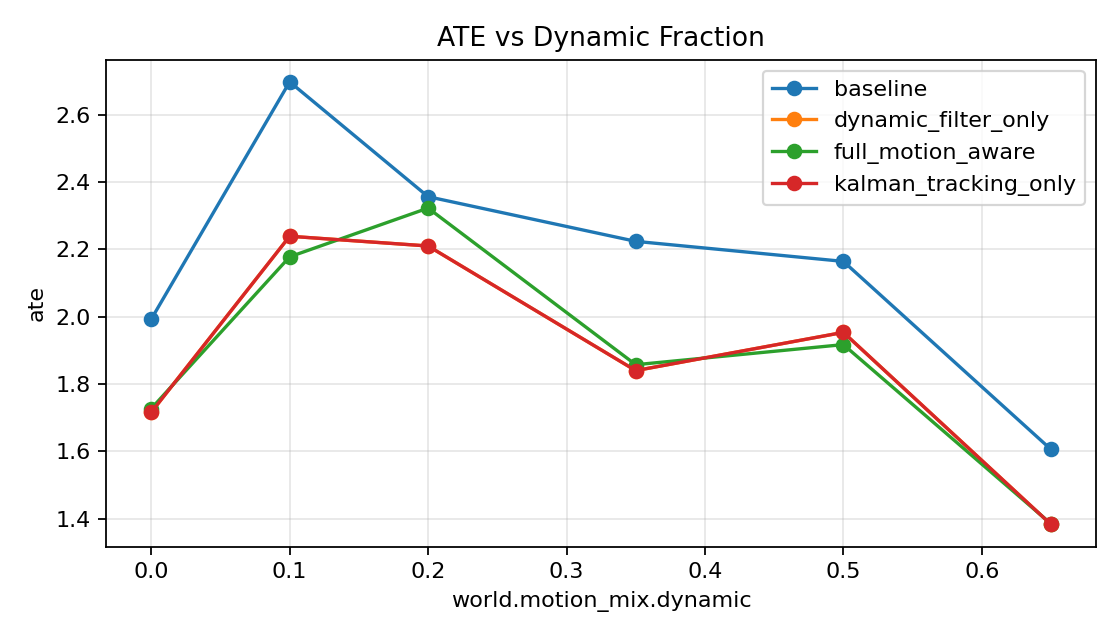
\includegraphics[width=\linewidth]{stress_dynamic_fraction.png}
    \caption{ATE versus dynamic-object fraction.}
\end{subfigure}
\hfill
\begin{subfigure}{0.48\linewidth}
    \centering
    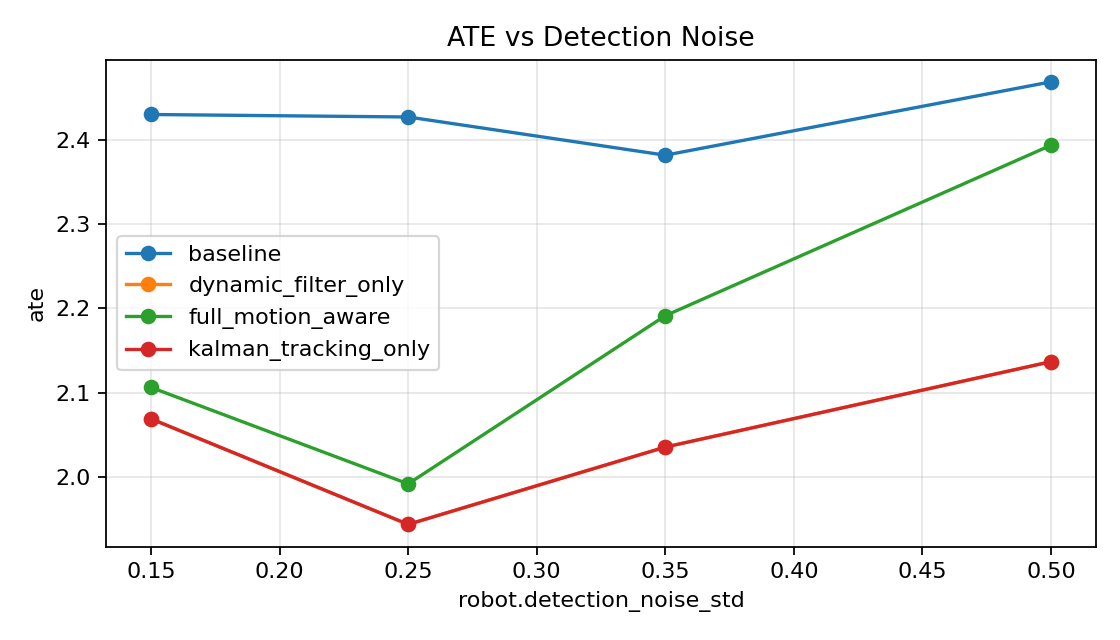
\includegraphics[width=\linewidth]{stress_noise.png}
    \caption{ATE versus detection noise.}
\end{subfigure}
\caption{Stress-test curves for dynamic clutter and observation noise. Lower ATE is better.}
\label{fig:stress_plots}
\end{figure}

\begin{figure}[t]
\centering
\begin{subfigure}{0.56\linewidth}
    \centering
    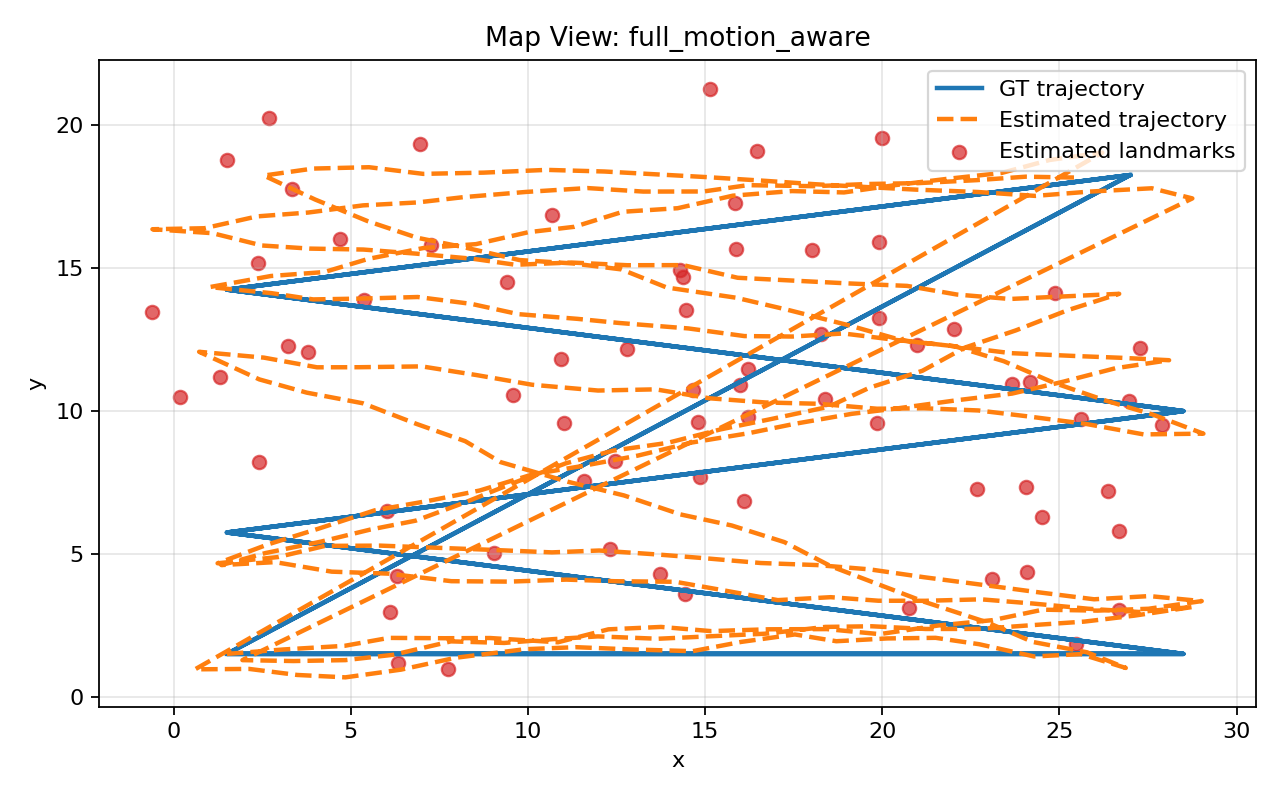
\includegraphics[width=\linewidth]{full_motion_aware_map.png}
    \caption{Full motion-aware map and trajectory view.}
\end{subfigure}
\hfill
\begin{subfigure}{0.38\linewidth}
    \centering
    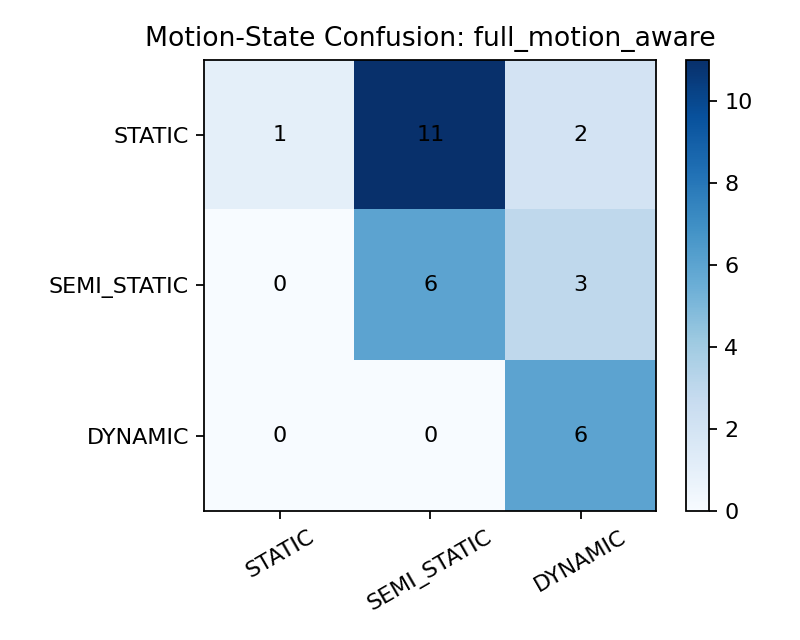
\includegraphics[width=\linewidth]{full_motion_aware_confusion.png}
    \caption{Full motion-aware state confusion matrix.}
\end{subfigure}
\caption{Qualitative outputs for the full motion-aware method. The accompanying animation is saved as \texttt{full\_motion\_aware\_animation.gif}.}
\label{fig:qualitative}
\end{figure}

\section{Discussion}
\subsection{Why the extension works in simulation}
The experimental improvements are consistent with the theoretical argument. POV-SLAM-style consistency reasoning is well suited to semi-static changes because it can reduce the influence of unreliable object-map associations. However, continuously dynamic objects create a repeated stream of inconsistent landmark observations. If they are only represented as unreliable landmarks, they can still consume association capacity, create unstable map hypotheses, and reduce the clarity of the object map.

The motion-aware extension changes this behavior by giving dynamic objects their own representation. Dynamic detections are not forced into the stationary landmark map. Instead, they are tracked with a motion model and visualized as moving entities. Static and semi-static objects remain available for localization and map updates. This separation improves ATE in the tested benchmark families and also makes the qualitative outputs easier to interpret.

\subsection{Why the full method is not always the lowest-ATE method}
The dynamic-filter-only ablation is often the best ATE performer. This is not a failure of the concept; it is a useful diagnostic. In the current lightweight backend, the Kalman tracker is a sidecar module. It improves dynamic object interpretation, but it does not participate in a full joint factor graph over robot poses, static landmarks, semi-static relocation hypotheses, and dynamic object trajectories. Therefore, the main localization benefit comes from the simplest part of the extension: excluding dynamic objects from stationary landmark correction.

A stronger future system would make dynamic tracks explicit optimization variables. The graph would include static landmark factors, semi-static relocation factors, dynamic motion-model factors, detection-to-track factors, and robot-pose factors. Such a formulation could allow reliable moving objects to help constrain ego-motion when static support is weak, but only through a principled joint optimizer. The present prototype intentionally stops short of that complexity.

\subsection{Limitations}
This report should be read as a controlled simulation study, not as a real-world SLAM benchmark. The main limitations are:
\begin{itemize}[leftmargin=*]
    \item the environment is 2D and object-level only;
    \item observations are simulated detections rather than raw visual features;
    \item the baseline approximates POV-SLAM's semi-static consistency behavior but does not reproduce its full factor-graph variational EM implementation;
    \item the motion-aware method uses heuristic state classification rather than learned perception;
    \item dynamic tracks are not jointly optimized with robot poses;
    \item the reported figures and metrics are generated from a small controlled simulation suite.
\end{itemize}

These limitations are acceptable for the stated goal: demonstrating the idea in a reproducible simulation-only prototype. They also define a clear path for future work.

\section{Conclusion}
This project extends a POV-SLAM-style semi-static object-aware SLAM baseline with explicit motion-state reasoning. The baseline captures the key POV-SLAM idea that object consistency should be estimated probabilistically so that semi-static changes do not corrupt localization and mapping. The proposed extension adds a three-state layer that distinguishes static landmarks, semi-static relocated objects, and continuously dynamic objects. Dynamic objects are excluded from stationary landmark updates and tracked separately with a constant-velocity Kalman filter.

In the current 2D simulation benchmark, the motion-aware variants improve ATE relative to the simplified POV-SLAM-style baseline across mixed, semi-static-only, dynamic-fraction stress, and noise stress experiments. The pure filtering ablation provides the strongest localization improvement, while the full motion-aware system provides the richer scene interpretation required for report-quality qualitative visualizations and future dynamic-object SLAM extensions. The main conclusion is that explicit dynamic-state separation is a legitimate and useful extension to POV-SLAM-style semi-static reasoning, especially in environments where continuously moving objects coexist with long-term semi-static changes.

\appendix
\section{Reproducibility Commands}
From the project root, activate the virtual environment and run:
\begin{verbatim}
source .venv/Scripts/activate
python scripts/run_experiments.py --config config/experiments.yaml
python scripts/plot_results.py --metrics-dir outputs/metrics --method full_motion_aware
python scripts/view_run.py --run outputs/runs/default_mixed_demo_full_motion_aware_seed7.json
\end{verbatim}

\section{Report Build Command}
If a LaTeX distribution is installed, build from the \texttt{report/} directory:
\begin{verbatim}
pdflatex main.tex
bibtex main
pdflatex main.tex
pdflatex main.tex
\end{verbatim}

\bibliographystyle{plain}
\bibliography{references}

\end{document}
